% Chapter 1

\chapter{An introduction to biodiesel} % Write in your own chapter title
\label{Chapter1}
\lhead{Chapter 1. \emph{Biodiesel}} % Write in your own chapter title to set the page header


\section{Resources}

A midden is an archaeological feature of prehistoric human life, consisting of all the stuff that a household or community discarded, all on a pile. The excavation of middens can tell archaeologists a lot about diets and customs of prehistoric people.

The midden is a sign that humans have, since the dawn of civilisation, had a problem with discarding of the remnants of resources. Today we  might not have the same problem near our homes, but our landscape is littered with mine dumps and ash dumps from power stations. We use up resources and the waste of that usage alter our world.

The discovery in the 1800s of the internal combustion engine and the discovery that it can be fueled by plentiful and cheap petroleum might have seem like a break from this cycle. The oil was pumped from the ground, and after processing all of it was used in engines, and the remnants was a gas that was exhausted into the air and disappeared. 

But the sad thing was, this didn't work for very long. The carbon cycle had been elucidated by Priestly in 17xx, and it was soon realized that the carbon dioxide would build up in the atmosphere. Arrhenius was the first to make the connection between the rising carbon dioxide levels in the atmosphere and a possible increase in the atmospheric temperature.

\section{Introduction to Biodiesel}

Biodiesel is a diesel fuel, in other words it is a fuel for compression-ignition internal-combustion piston engines. It is derived from fats and oils, and is therefore biologically based. Because plants and animals obtain their fats and oils from photosynthesis biodiesel has the potential to be a carbon-neutral fuel, which is to say it is one that will not contribute greenhouses gases to the atmosphere.

While diesel engines can be run on vegetable oils directly, there are technical problems associated with it. However, the conversion of the triglycerides of the oil to a mixture of fatty acid esters is a simple reaction, well understood, and easy to implement. This reaction is known as a transesterification, since the glycerol ester of the fatty acids is turned into a methanol ester. 
\begin{figure}[htbp]
	\centering
	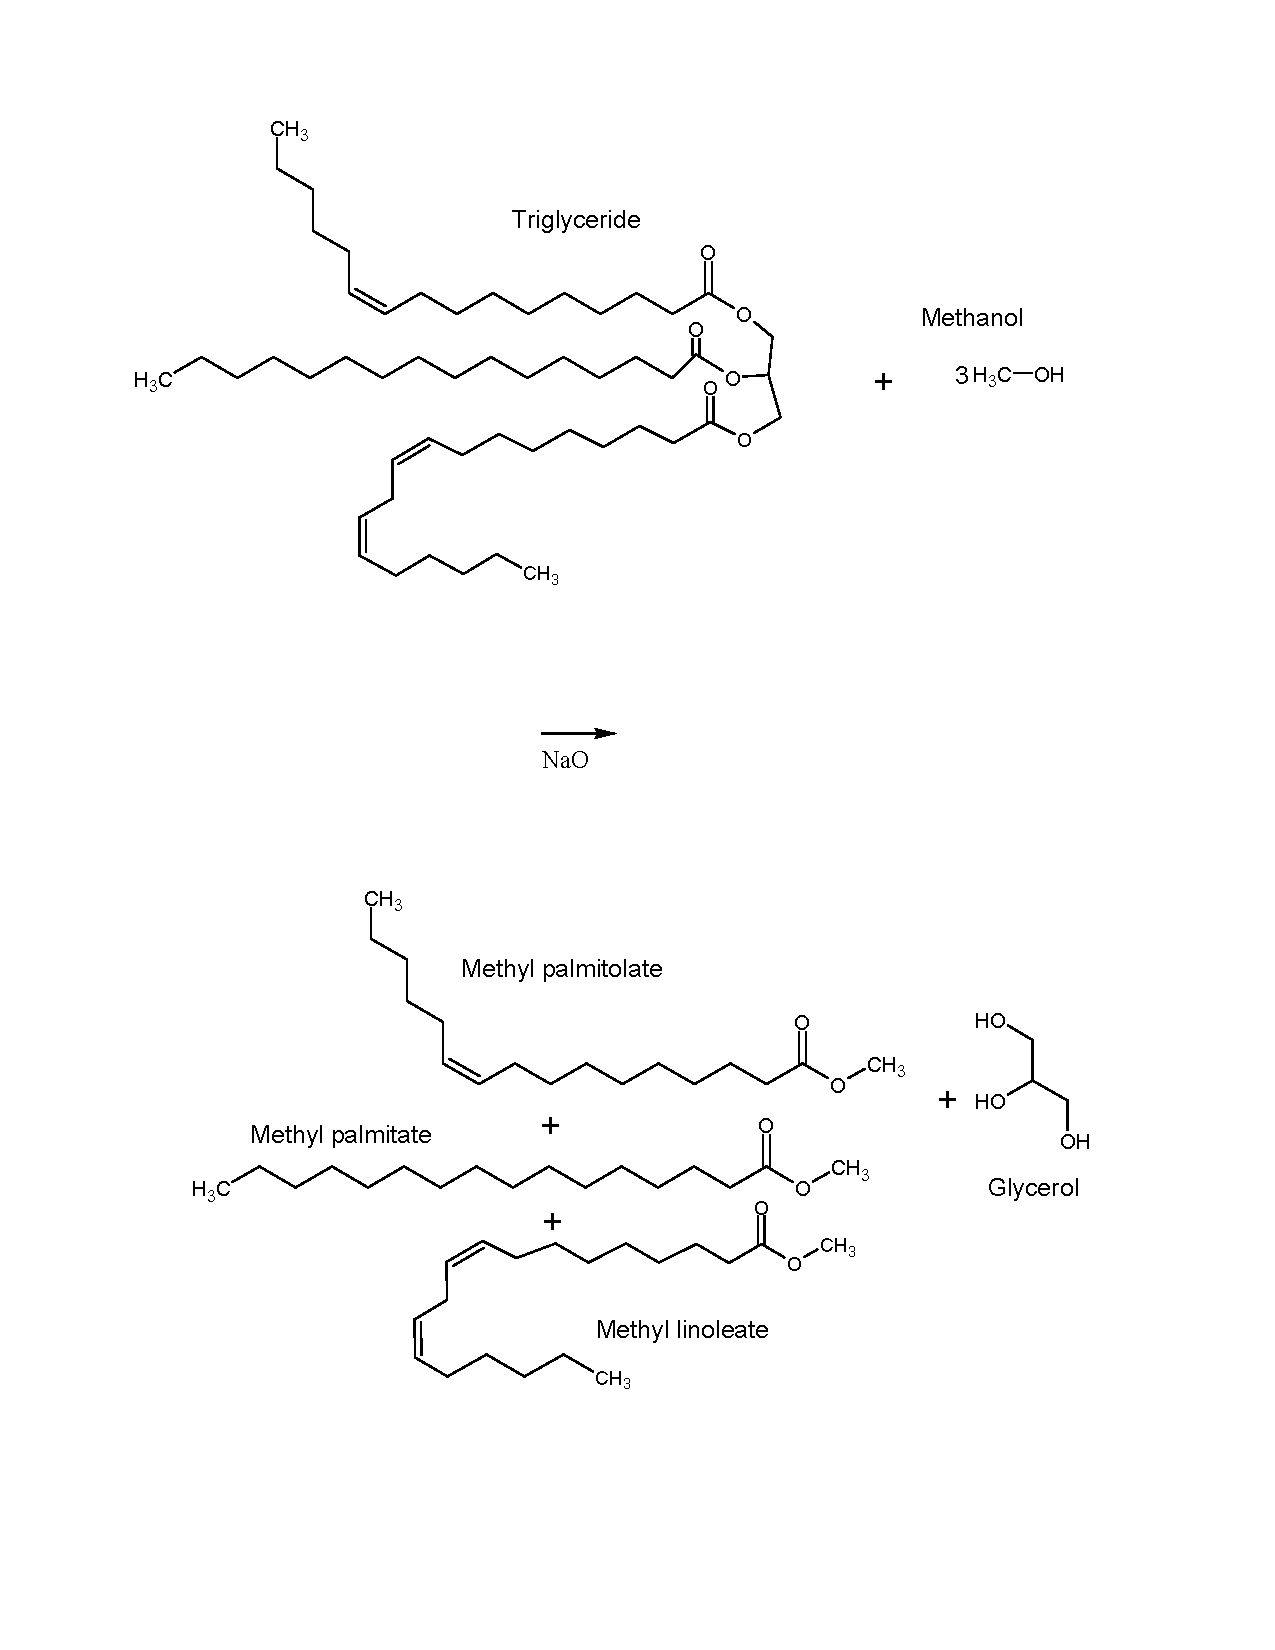
\includegraphics[width=0.8\textwidth,natwidth=4.17in,natheight=3.32in]{./Figures/Transesterification.pdf}
	\rule{35em}{0.5pt}
	\caption[Transesterification]{Transesterification of acyl triglycerides.}
	\label{fig:Transesterification}
\end{figure}

This transesterification turns the oil into a mixture of fatty acid esters that has a lower viscosity and other physical properties that makes it suitable for use as a diesel fuel. 

There are a few things to note about this picture:
\begin{itemize}
	\item Some of the fatty acids have double bonds, some not. In general, the fewer the number of double bonds, the easier it is for the straight chains to crystallize, and by implication, the higher the melting point. 
	\item The fatty acid chains can have different lengths. In common fats and oils the number of carbon atoms vary between 12 and 20. The longer the chain the higher the melting point.
	\item The different fatty acids can sit on different positions on the glycerol backbone.
	\item.Each fat molecule can have different 
	\item It is a three-step reaction, and production is thermodynamically controlled. Therefore there are intermediates in the reaction mixture, also diglycerides and monoglycerides.
	\item The polar methanol reagent and the nonpolar oil or fat are not miscible, and neither are the glycerol and the FAME products. Therefore the reaction needs mixing for the reaction to take place, but also waiting for the products to separate, and the reaction mixture is usually heated to reduce the viscosity and facilitate mixing. 
	\item The reagents and the products are miscible. Since the reagents can't be tolerated in the product, this implies that the reaction must be pushed to completion by choosing appropriate reaction conditions. 
	\item The methanol reagent is very inexpensive because it is usually obtained from the petroleum industry. This portion of the biodiesel is therefore not carbon neutral. 
	\item The glycerol is a side product with very little value, and at the moment it needs to be disposed of. 
\end{itemize}



\section{Biodiesel production}

The basic transesterification reaction of biodiesel is quite simple. The feedstock fat or oil is mixed with an excess of methanol, and a catalyst is added, and the reaction mixture is heated and stirred. Under these conditions the equilibrium of the transesterification reaction lies far over to the product side of the reaction, and the biodiesel is formed. The reaction products, glycerol and biodiesel, are also not miscible, and the two separate into layers, FAMEs at the top and the glycerol at the bottom. The glycerol is drained off and the biodiesel is washed with water to remove catalyst remnants and methanol. 

The feedstock of biodiesel can be almost any fat or oil. Vegetable oils are preferred, because they can be farmed. Animal fats can be used, and from a dietary point of view the reduction of animal fats in the national diet would improve public health, the carbon intensity of the production of animals is very high, and more carbon emission reduction can be achieved by not breeding animals than by using their fats as fuel. At best, animal fats as feedstock should be seen as a sink for waste animal products. A recent example of this is a proposal to render the daily 8 tonnes of chicken carcasses from the daily natural deaths of layer chickens in the Namakkal district in Tamil Nadu state in India, which could deliver enough rendered chicken oil produce 800000 litres of biodiesel per year. (There is already a ready market of chicken meal for feed and fertilizer.) \cite{Abraham2013} \cite{Ananth2013}

Not all feedstocks are created equal. The promotion of biodiesel is a political tool, and therefore some are considered better than others. in the USA soybean oil is the main feedstock, mainly because the National Biodiesel Board is controlled by soy interests, and owns the safety data that allows certified biodiesel to be sold on the open market\cite{Estill2005}, keeping other feedstocks out of the market. In Europe, especially Germany, rapeseed oil is the main feedstock, because it keeps German farmers on their land. The European order of things is a bit more democratic, so anybody who can produce biodiesel from any feedstock, although some are less likely to receive government support than others.

One of the few undoubtedly good feedstocks of biodiesel is used vegetable oil. Vegetable oils that are used for frying food deteriorate with use, and good practice, enforced by many governments, don't allow the oil to be used for food beyond a certain point. Ordinarily this oil would then be discarded in landfill, were it would eventually be broken down by microorganisms to carbon dioxide and water. But the used oil can be collected by the biodiesel industry and converted into fuel, which can then power vehicles. 

This sounds like a good idea, except that the soap industry also depends on waste vegetable oils and waste fats. Lacking a source of oils for the cosmetic and cleaning industry, they might turn to synthetic surfactants, wholly made from fossil carbon.

The catalyst most often used in the transesterification is sodium hydroxide or sodium methoxide. This is the cheapest available catalyst. Unfortunately the spent catalyst is also a waste product, and it contains sodium. For countries near the sea the sodium waste is not a problem since they can pump it into the sea with little concern. In South Africa, the disposal on land of sodium is forbidden, so disposal becomes a huge cost. Acids catalysts are also used, and have the added benefit that they will esterify free fatty acids, but the reaction is much slower than that of the base catalysis. In an industry where most reactions are done in batch conversions the slowness is undesirable.

There is a lot of research being done on heterogeneous catalysts for biodiesel. In general, however, the catalytic efficiency is low, and not all of the oil gets converted, and the catalysts need to be regenerated. In the style of catalyst development this is nothing new, and without doubt the quality of the catalysts will improve as time goes by, but

Another promising development in biodiesel production is the use of supercritical methanol. In supercritical methanol the methanol is at high pressure and temperature, and the properties of it change, so that it becomes a solvent for the feedstock oil. The reaction can then take place in a homogeneous mixture, which speeds up the reaction considerably, because the rate-limiting effect of mass transfer across a phase interface is eliminated. When the pressure in the reaction vessel is released, the solvent properties of the methanol change again, and the biodiesel and the methanol/glycerol solution separates. The methanol and the glycerol can be separated by a simple distillation, and there is no spent catalyst to get rid of. 

Feedstocks contain different contaminants. Free fatty acids is one common one, because in any oil there are some free fatty acids. An abundantly available feedstock, rice bran oil, is not used for biodiesel because of the high level of free fatty acids. Although there are technological fixes for this, the increased complexity in the production process increases the price of the biodiesel, making it uncompetitive with petrodiesel.

Most feedstocks also contains other, non-oil lipids. The tocopherols is one, a common natural antioxidant found in cell membranes. This might provide an antioxidant effect to the biodiesel too. The phospholipds that make up cell membranes are also present, and because they have a detergent effect are sometimes a major problem. Biodiesels often retain the colour of their parent feedstock, because the pigments that provide the colour are perfectly oil-soluble, and are equally at home in the feedstock oil and the finished biodiesel.

\section{The chemical analysis of biodiesel and SANS 1935}

While the fuel industry had some time to get used to the requirements posed by a good diesel fuel, and some of those can be carried over to biodiesel, biodiesel and petrodiesel are very different chemical mixtures, and consequently have different requirements.

In response to this, there had been starts made to setting up standards of good biodiesels. The Americans have the ASTM D6751, and the Europeans wrote EN 14214. Interestingly, the US standard only cover biodiesel as a blend feedstock, while the European standard applies to biodiesel as both an ``extender'' and a pure fuel. 

In South Africa SANS 1935 \cite{SANS1935} was adopted. This is essentially a copy of the European standard, with minor adjustments made to accommodate the most likely South African feedstock of large-scale biodiesel production, soybeans.

Below follows a point-by-point explication of the meaning and implications of the content of SANS 1935

\subsection{1 Scope}

This paragraph explains the scope of the standard, \textit{i.e.} that it applies to biodiesel, which is a diesel fuel or a diesel fuel blend component.

\subsection{2 Normative references}

This section contains a long list of standards referred to in this method. 

\subsection{3 Definitions}

This short section defines two terms: \textbf{additive} and \textbf{ biodiesel}.

\subsection{4.1.1 The automotive biodiesel fuel shall contain, principally, mono-alkyl methyl esters of long chain
fatty acids derived from vegetable oil.}

This clause pins biodiesel down as quite a particular product. While this makes it easier to write the standard, it also might stifle innovation. Specifying methyl esters, for instance, precludes the use of ethanol as alcohol in the transesterification. It's a fact not often mentioned in the discussion of biodiesel as a green product that the methyl group in the biodiesel molecule is practically universally derived from the petroleum industry. Its low price and abundant availability make a hard economic argument against the adoption of another alcohol, but while this is the case biodiesel cannot be described as a sustainable fuel. 

The phrase mono-alkyl methyl ester is not a good phrase to use, and I believe it to be the result of an editorial mishap. 

\subsection{4.1.2 Suitable fuel additives without known side effects may be used to help avoid deterioration of
driveability and emissions control durability. Other technical means that exhibit an effect equivalent to
that of additives can also be used.}`

This clause enables manufacturers to invent modifiers to give the fuel more desirable properties.

\subsection{4.1.3 The fuel may contain small quantities of colouring materials which are documented as harmless
to give it a distinctive colour.}

This clause allows manufacturers to differentiate products, help prevent mistakes, and is sometimes used to identify fuel, \textit{e.g.} fuel with a different taxation rate.

\subsection{4.1.4 The fuel shall be clear and free of visible water, sediment, suspended matter and any other
contaminant that is documented as likely to cause malfunctioning of equipment designed to use this
type of fuel, either as a blend or in its 100 \% concentration form.}

This is just stating the obvious, in effect declaring that a fuel sold as biodiesel is fit for use, and also provides blanket protection against contaminants not otherwise specified.

\subsection{4.2 Physical and chemical properties
The fuel shall comply with all the requirements given in table 1.
NOTE 1 In case of a need for identification of biodiesel, it is recommended that a method based on the
characterization of fatty acid methyl esters by LG/GC, in accordance with EN 14331, be used.
NOTE 2 In case of a need to identify the source oil of biodiesel, the iodine value of the biodiesel can be calculated
by the method presented in annex B.}

This sort paragraph is actually the meat of the standard. It refers to Table 1 of the standard, which is discussed in detail on page \pageref{table1} below.

\subsection{5.1 For all tests, use samples taken in accordance with annex D.}

This draws attention to the fact that doing chemical tests for commercial purposes need to ensure that the sample is actually representative of the bulk. It would be easy to take a single sample from a bulk container in such a way that it would be sure to pass or fail the test. For example, a bulk fuel tanker could contain a minuscule amount of water at the bottom of the tank. If a simple sample were to be taken by means of a draining cock, this small sample would contain a relatively large amount of water, violating the standard, while the bulk of the sample might actually be of very good quality. A representative sample would provide a meaningful average of the whole. 

\subsection{5.2 For all properties, use the applicable test method or, when relevant, one of the applicable test
methods listed in column 3 of table 1}

This points to the fact that standardized methods should be used, and that not all tests are equal in accuracy and precision.

It also protects the testing laboratory, because if a new problem should be developed with the fuel's quality assessment, and the problem had not become apparent in well-performed analytical tests specified by the standard, the laboratory would have performed all the legal steps to ensure quality. Ethical considerations would have to be considered on a case by case basis, because a problem with a fuel might have been apparent to test laboratory staff that did not show up in the tests.
	
\subsection{5.3 The limiting value for the carbon residue given in table 1 is based on product prior to the addition of ignition improver, if used. If a value exceeding the limit is obtained on finished fuel in the market, use ISO 13759 to determine the presence of a nitrate-containing compound. If an ignition improver is thus proved present, the limit value for the carbon residue of the product under test cannot be applied. The use of additives does not exempt the manufacturer from meeting the requirement of maximum 0.30 \% mass fraction of carbon residue prior to the addition of additives.}

This is a methodical sidestep of a known chemical interference that cannot be controlled for using existing methods.

\subsection{5.4 Precision and dispute}

This section talks about precision, and how dispute should be resolved. Discussion of it falls beyond the scope of this chapter.

\subsection{6 Packing, marking and placarding}

This section deals with the packing of biodiesel in containers. Basically it should be packed in drums and tanks that does not leak, the tanks and drums should be labelled properly, and that road freight standards apply if biodiesel is transported by road. (I wonder why transport by rail is not mentioned. Is this oversight, ignorance, or does the railway apply its own standards? In any case it seems a bit like the highly efficient (in terms of carbon emissions) train transport system is being ignored again)

\subsection{Annex A: Precision data}

Any test method yields a result, with the result being true only to a certain degree. This degree of trueness is given by the precisions. This table is included because the precisions given for the established standard values might differ slightly if it is applied to other materials.

\subsection{Annex B: Calculation of iodine value}

Iodine value is a very old technique for determining the degree of unsaturation of fats and oils. I have the feeling that somebody on the committee, some crotchety oldster, insisted on including iodine value in the table of specified values. The younger and more advanced members of the committee added this annex to get something more advanced in. ``In the case of dispute on the iodine value this method shall be used as a substitute for EN 14111''. This sentence seems to indicate that chromatographic technique specified here is superior to the iodine value method. 

Of course the iodine value of EN 14111 is simpler to implement than the chromatographic method of EN 14103, but since EN 14103 will be performed in any case, the redundancy doesn't seem to make sense. Knothe \cite{} seem to think so too.

\subsection{Annex C:(normative) Correction factor for calculation of density of biodiesel}

This correction is an aid to the testing lab. It is much easier to measure a density at an unspecified (but fixed) temperature than it is to do it at a specified temperature. This correction makes it easier to apply the test.

\subsection{Annex D: (normative) Sampling and compliance with this standard}

This annex provides the technical details of the section 5.1 of the standard.

\subsection{Annex E: Quality verification of automotive biodiesel fuel}

This Annex is an advertisement for the ISO 9000 quality assurance system.

\subsection{Table 1}

Here follows a detailed discussion of the contents, relevance and methods of Table 1 of SANS 1935.
\label{table1}
\subsubsection{Ester content}

This is the ester content specified: 96.5\% This does not leave much space for other stuff, but leaves some room for contamination of fuel-valued components. It is interesting that this line does not specify that the esters should be methyl esters, but that is covered in section 2.1 of the standard. The footnote specifies that the other 3.5\% may only be additives, and not any non-FAME material.

\subsubsection{Density}

The fuel's density is specified, as the mass per unit volume. This is necessary, because fuel quantities can be specified in either volume or mass, and there needs to be a good relationship between the two. 

The density of the fuel also determines its energy density.

\subsubsection{Kinematic Viscosity}

This is a very important specification. 

The kinematic viscosity of a liquid is its viscosity divided by its density. This gives a number that can be used in calculating its flow properties under dynamic conditions.

If the viscosity is too high, the injectors in the engine might not be able to inject the right amount of fuel, because of the metering of the pump is based on timing, and if the flow is not as expected the metering will not be as expected.

If the viscosity is too high, the droplet-forming mechanism is not as effective. In this process, surface tension of the liquid fuel pulls the droplets into spherical shape. The faster the surface tension can act, the smaller the droplets can be. The rate of flow of the liquid is limited by its viscosity, which makes a defined viscosity necessary for the proper operation of the engine.

If the viscosity is too low, there might be other problems. The injection process in the diesel engine uses very high pressures to produce a fine enough spray of fuel into the combustion chamber. While a lower viscosity is preferable for producing a better spray, once again the volume delivered is measured by time, and if the flow is higher than expected, the amount of fuel will be too much. There is also the problem of reverse flow. In the injector the piston of the pump is not sealed, because it is not usually necessary, so it is not a positive displacement pump. If the viscosity of the fuel is too low, more fuel than expected will flow past the injector piston back into the system, and less will be injected into the engine. This problem would not apply to common-rain engines.

Nevertheless, the range of viscosities are large enough to accommodate a wide variety of feedstocks to be used, from heavy palm oil to light sunflower oil.

\subsubsection{Flash Point}

The flash point of a flammable liquid is that temperature of the liquid where a flame applied to the vapour above the liquid is transferred to the liquid itself.

The flash point of biodiesel is naturally much higher than petrodiesel. In the manufacturing process, however, there might be highly flammable methanol left in the final biodiesel product, which would decrease its flash point dramatically. 

\subsubsection{Sulfur Content}

One of the pollutants from petrodiesel, and from coal and petroleum combustion in general, is sulfur dioxide. When this mixes with rainwater it forms sulfurous acid, and acidifies the rainwater, forming what is known as acid rain. This is toxic to plants and has the potential to damage ecosystems. Legislation and regulation have steadily decreased the permissible amounts of sulfur emissions. This is fairly easy to implement in stationary plants such as power stations, but in vehicles it prove to be more expedient to limit the amount of sulfur in the fuel, regulating the emissions that way. South Africa has only recently introduced low-sulfur diesel.

Biodiesel is naturally sulfur-free, so this limit would mostly prevent the use of sulfur-containing additives, and the occasional odd feedstock with high sulfur content.

\subsubsection{Carbon Residue}

Biodiesel is a fairly non-polar liquid, and therefore a good solvent for other compounds. Some of these compounds might be solids, so that when the fuel evaporates there may be a residue. These solids could tend to accumulate in some part of the fuel system or engine, causing improper function or damage. (Note that the carbon residue have a fuel value, and its presence does not detract from the biodiesel's value as a fuel.) This test puts a limit to these dissolved solids. 

\subsubsection{Cetane Number}

This number points to the fuel's suitability as a diesel fuel. At a low cetane number, the fuel evaporates and ignites too easily, causing detonation, called pinging or knocking. Beyond a certain cetane number, however, there is no change in performance.

The cetane number is usually determined in a test engine, and this is a fairly specialized test.

\subsubsection{Sulfated Ash Content}

Ideally a fuel will burn completely into gaseous compounds, and if it were composed entirely of carbon compounds and the combustion process was perfect it would. However, the feedstocks of biodiesel naturally contains some non-carbon compounds, and these will not necessarily vaporize during combustion. This would then remain in the engine, possibly causing deposits, altered operation and possibly damage.

In this test a sample of the fuel is digested with sulfuric acid, and the remnants heated. The remains is ash, and represents the non-combustible portion of the fuel. This paragraph specifies a limit to ash.

\subsubsection{Water Content}

Water in fuel is of great concern. In combustion it robs energy, in storage it promotes corrosion, it permits growth of bacteria, in increases solubility of ash-forming compounds.

Biodiesel is more hygroscopic than petrodiesel, and therefore the limits on water need to be set stricter.

Water in biodiesel can be determined by the Karl Fischer titration usually used in petroleum analysis.

\subsubsection{Total Contamination}

I don't know what this means. It seems to be taken over from the petrodiesel methods. The standard notes in a footnote that ``Pending development of a suitable method, EN 12662 shall be used.'' This seems to show that it is not deemed very important, but worth looking at.

I suppose the total contamination would be all the things in the fuel that are not FAMES or additives.

\subsubsection{Copper Strip Corrosion}

In this test clean copper strips are immersed in the biodiesel for three hours at 50 $^\circ$C. After this time the copper strips are visually inspected, and the amount of corrosion judged, compared to standard strips. This is a practical test of the corrosive properties of the biodiesel. If the fuel causes excessive corrosion in fuel systems it could cause leaks in storage tanks and transfer lines, and in the engine it could lead to excessive wear and engine failure.

\subsubsection{Oxidation Stability}

Biodiesel should be stable against oxidation in the air. This is a measure of its shelf life. Oxidation of the biodiesel causes the chemicals it is made of to change its composition, and therefore it might no longer conform to specification. Oxidation of the fuel increases its acid value and increases the cetane number, but otherwise it has little impact on the usability of the fuel.

The oxidation stability is another practical measure. It is done in an apparatus called the Rancimat. In this apparatus the sample of biodiesel is heated while a stream of oxygen is bubbled through. The air stream is captured from the sample and then bubbled through water in a conduction cell. The conduction in the conduction cell depends on the volatile polar compounds give off by the heated sample. Under ordinary circumstances there are no volatile compounds coming off biodiesel. With time and heat, however, the sample starts to oxidize, and some of the oxidation products are volatile and polar, and in addition, catalyses the oxidation. After an induction period therefore, oxidation starts and rapidly accelerates. This oxidation can be observed as a sudden increase in the conductivity of the water in the conductivity cell.

This method and apparatus has been transferred from the food industry, where it has been used in the determination of the resistance to oxidation of fats and oils.

It is fairly important that biodiesel have a good stability at high temperatures too. In modern common-rail engines the diesel fuel is circulated in the injection system on or near the hot engine block, and the fuel might stay at these high temperatures for an appreciable time before it is injected.

\subsubsection{Acid Value}

The acid value gives an indication of the acidity of the biodiesel. High acidity is of course associated with high corrosion.

The cause of too-high acidity can be either left-over acid catalyst, or by high levels of free fatty acids. Some biodiesel feedstocks, like rice bran oil naturally contains many free fatty acids. Free fatty acids are also a source of carbon residue, because they are non-volatile: some of them are even solids at room temperature.

\subsubsection{Iodine Value}

The iodine value of the biodiesel is a measure of the degree of unsaturation of the fatty acids of the biodiesel. As discussed above, the inclusion of this measure in the standard is of doubtful utility. Perhaps it was introduced to protect the European rape seed farmers from the possibility of the importation of cheap soy-based biodiesel from the USA, because the limit in the original European standard is much lower than in the South African standard, where it had to be increased to accommodate the likelihood of soybean-based biodiesel. 

On the other hand, the setting of this value has made palm oil (which is a highly saturated oil) a good feedstock for European biodiesel, and therefore tropical countries have started to produce palm oil specifically for the European export market. This is unfortunate, for in some countries, Malaysia being a prime example, rainforests were being replaced by oil palm plantations.

\subsubsection{Linolenic acid methyl ester}

Linolenic acid is a doubly-unsaturated fatty acid with a chain of 18 carbon atoms. Its methyl ester is a valid compound in the fuel, and therefore the limit is very high at 12\% mass fraction. However, because of the double unsaturation including an allylic carbon atom it is especially vulnerable to oxidation. Keeping the quantity of this FAME low helps promote a stable fuel with a long shelf-life.

The specification of linolenic acid in this context is unfortunate, because it is not the only unstable fatty acid with allylic double bonds. It might therefore be possible to produce an unstable fuel that conforms to the specification. 

\subsubsection{\texorpdfstring{Polyunsaturated ($geq$ 4 double bonds) methyl esters}{Polyunsaturated methyl esters}}

No more than 1\% of the FAMEs in biodiesel may have more than four double bonds. This is once again a matter of stability and shelf-life, and therefore the limit is set very low. 

It is also to prevent fish oil from being used as a feedstock for biodiesel production. This is a good thing, because the world's fisheries are in a perilous state, and to allow fuel for an excessive lifestyle to be produced from this scarce resource would be near criminal.

It is interesting to note that this limit is one for which no test has been prescribed, because none exists yet.

\subsubsection{Methanol content}

No more than 0.2\% of the biodiesel may be methanol. Methanol is one of the feedstock products in biodiesel production, but it adversely affects the performance of the fuel. It lowers the viscosity and the flash point and decreases the cetane number. It might mask viscosity problems, which would appear if the methanol evaporated during storage.

Besides, the methanol is one of the non-renewable portion of the fuel, so it should be used very sparingly.

Ordinarily there would not be much methanol left in biodiesel, because it separates from the biodiesel and up in the glycerol layer. An excess of methanol in the finished biodiesel would indicate some emulsifying effect of some contaminant, or another chemical problem with the fuel.

\subsubsection{Monoglyceride content}
\subsubsection{Diglyceride content}
\subsubsection{Triglyceride content}

These three go together. The reaction of the production of biodiesel is a three-step reaction, where the three fatty acids attached to the glycerol backbone are picked off one by one and methylated. 

Like this: 	\\Triglyceride + MeOH $\rightarrow$ Diglyceride + FAME\\
		Diglyceride + MeOH $\rightarrow$ Monoglyceride + FAME\\
		Monoglyceride + MeOH $\rightarrow$ Glycerol + FAME 
		
Because these are equilibrium reactions, there are always some of the starting compounds left in the final mixture. The mono-, di- and triglycerides are besides this also soluble in the FAMEs. This makes a great possibility for contamination by these side-products. This then also test is also a test to make sure that the reaction had run to completion.

These are also the compounds that are responsible for injector coking and other problems, so their control is important. 

Because the last is the one that is most difficult to drive into an equilibrium where the products are in excess, the limit on monoglycerides (0.8\%) is higher than the 0.2 \% limit for the tri- and diglycerides.

\subsubsection{Free glycerol}

Glycerol is the side-product of the reaction, and it is definitely not a wanted compound in biodiesel. It increases the viscosity of the fuel and makes it more hygroscopic. It provides nutrients for organisms like algae and bacteria that colonizes fuel tanks.

As can be expected from the number of hydroxyl groups that can form strong hydrogen bonds, glycerol is denser than the FAME esters, and separates out under gravity. If not enough settling time is allowed, though, or there is a problem with emulsification, the glycerol content of the biodiesel may exceed the low 0.02 \% limit.

\subsubsection{Total glycerol}

Total glycerol includes the free glycerol and the glycerol bound to the mono-, di-, and tri-glycerides. Since this limit is quite high (0.25 \%) compared to the 0.02 \% in the Free Glycerol test, it seems that bound glycerol is much more tolerable. 

Including total glycerol seems redundant, because the limit would never be reached if all the glycerides are under control.

\subsubsection{Group I metals (total of Na and K)}

Fatty acids that are neutralized by alkali bases form soaps. These are molecules that consists of a fatty acid conjugate base and an alkali metal atom. These are not particularly soluble, promotes the forming of emulsions and increases ash content. 

Of course sodium and potassium hydroxide are used in the base catalysis of the transesterification process. 

The problem with fatty acids are that they form a natural component of many feedstocks, and that soap formation is then a natural side-product of the transesterification. The free fatty acids can be esterified in a separate acid-catalysed process. This play some role in the economics of biodiesel, because it makes low-FFA feedstocks desirable.

\subsubsection{Group II metals (total of Ca and Mg)}

Calcium and magnesium hydroxides can also be used as catalysts, but are also naturally present in plants. The are also ash-forming compounds, so controlling for their presence.

Testing for these alkali and alkali earth metals are a test of sufficient washing of the biodiesel and the proper use of the correct amount of catalyst. 

\subsubsection{Phosphorous content}

I don't know exactly why the test for phosphorous, but it is a natural constituent of plants. Its oxides are acidic, so it will play a role in exhaust system corrosion if it got burned up in the engine. It will probably contribute to acid rain too, although the phosphorous compounds are not particularly volatile and therefore won't spend much time in the atmosphere.

\subsubsection{Cold Filter Plugging Point}

Petroleum products are mixtures, and therefore petrodiesel does not have sharply defined melting point. However, it does become solid at low temperatures, low being temperatures typically found in terrestrial winters. To ensure that the fuel remains liquid at all likely temperatures it us usual to specify some temperature above which the fuel should still stay liquid. 

Traditional measures include the ``cloud point'', the temperature where visible crystals first start appearing in the oil, giving it a cloudy appearance, and the ``pour point'', the temperature at which the oil can no longer be poured from a container. However, at the cloud point the fuel is still quite liquid, and usable as a fuel, so the cloud point does not give a good indication of suitability. So the compilers of EN 14214 settled for a more practical point, and uses the ``cold filter plugging point''. This is the temperature at which the biodiesel will contain enough solid material to plug a specified filter. This is used because the fuel system only need to pump the fuel through the fuel filter under cold conditions. 

In the European standard EN 14214 the temperatures and dates for which they apply are left to member countries to specify, since the standard needs to be applicable from Sicily to Finland.

SANS 1935, however has an easier task, and the cold filter plugging point (CFPP) is specified as -4 $^\circ$C in winter and +3 $^\circ$C in summer, and then goes on to say in a footnote. ``Winter shall be considered as being from 1 April to 30 September and summer shall be considered as being from 1 October to 31 March.''

\subsection{Conclusion}

The standard SANS 1935 then gives a long list of criteria to which a biodiesel must conform before it can be sold on the open market. There seems to be some redundancies and perhaps one or two contradictions in the standard, but in general the intent and its application is acceptable. It reflects the knowledge of the time it was written, and in future one will perhaps see an improved and more up-to-date version.

I will have to make a study of the numbers in the standard to see how they add up to a total biodiesel budget.

There is much that can be done to understand biodiesel chemistry better. The role of additives can be examined much further. Particular areas of concern are oxidative stability, where the use of anti-oxidants can be explored, and studies to understand the coking of injectors better

